\chapter{L'indice di vitalità}
\label{chap:vitalita}

Questo capitolo presenta l'indice di vitalità, formulato dal relatore come un indice che valuti quanto una persona si muove, oltre alla presenza sì o no. È la dimostrazione costruttiva che i dati del radar abilitano ciò che con un bit non è rappresentabile. L'algoritmo è stato specificato, corretto due volte sulla base dei dati, tarato su un sottoinsieme dei trial del Capitolo~\ref{chap:confronto}, validato su trial mai usati per la taratura, portato a bordo dell'ESP32 e verificato contro il calcolo di riferimento.

Il capitolo è organizzato come segue. La Sezione~\ref{sec:vitalita-motivazione} spiega perché la vitalità è una domanda diversa dalla presenza e come l'indice la rende leggibile. La Sezione~\ref{sec:respiro} mostra che il segnale su cui l'indice poggia contiene davvero il micro-movimento respiratorio, con una verifica a ritmo imposto. La Sezione~\ref{sec:vitalita-ingressi} descrive i dati di ingresso e l'algoritmo, insieme alle due versioni precedenti abbandonate, e la Sezione~\ref{sec:vitalita-classi} definisce le tre classi. La Sezione~\ref{sec:vitalita-taratura} riporta la taratura dei parametri e la validazione su trial separati e su una geometria diversa. La Sezione~\ref{sec:vitalita-bordo} descrive il porting sull'ESP32 e la verifica del calcolo a bordo contro quello offline, e la Sezione~\ref{sec:vitalita-limiti} chiude con i limiti, i casi limite e le possibili estensioni.

\section{Motivazione e presentazione}
\label{sec:vitalita-motivazione}
\label{sec:vitalita-presentazione}

Nel contesto del progetto la differenza fra presenza e vitalità è la differenza fra
due domande dei soccorritori. La prima è se c'è qualcuno sotto il banco, ed è la
domanda di presenza a cui rispondono gli obbiettivi O1--O3. La seconda è in che
condizioni si trova la persona. Se si muove attivamente è cosciente, se compie solo
micro-movimenti è ferita o intrappolata ma viva, oppure può non dare segni di
movimento rilevabili. Il PIR non può porsi la seconda
domanda, perché la sua uscita è un bit che non misura nemmeno la durata del movimento
(Sezione~\ref{sec:interpretazione-pir}). Il radar sì, perché espone l'energia riflessa per
gate di distanza, una misura continua di quanto si muove ciò che riflette. La
dose-risposta di Sezione~\ref{sec:dose-risposta} ha mostrato che questa grandezza è monotona
con la quantità di movimento (68,6, 84,4, 99,3 sui tre livelli a 1~m). L'indice di
vitalità sintetizza questa informazione in un numero fra 0 e 100, leggibile da un
operatore non tecnico, con una classificazione a tre livelli.

Una scelta di formulazione, concordata con il relatore, precede l'algoritmo. L'indice
non è descritto come misura del movimento toracico o rilevamento del respiro, ma come
indice generico di vitalità calcolato dall'energia radar. È la scelta più difendibile,
perché il respiro ha una sua verifica separata (Sezione~\ref{sec:respiro}) e l'indice è
definito per quello che calcola, cioè una funzione delle energie per gate del canale in movimento,
senza costruirvi sopra una misura fisiologica. Anche i nomi delle classi seguono
questo principio. Formule come ``poco vivo'' sono evitate, perché la classe descrive
il segnale e non l'individuo. I nomi adottati (vitalità bassa, moderata, alta)
qualificano l'indice, non la persona.

\section{Il rilevamento del respiro: una misura a sé}
\label{sec:respiro}

Prima dell'indice conviene mostrare che il segnale su cui poggia contiene davvero il
micro-movimento respiratorio. Il metodo segue la Sezione~\ref{subsec:corpo-immobile}. Si campiona
a 5~Hz un canale di energia per gate in engineering mode, si applica la FFT alla serie
temporale e si cerca il picco in banda 0,1--0,5~Hz. La frequenza del picco per 60 dà
gli atti al minuto. L'\ldb\ espone venti serie di energia e non tutte sono
utilizzabili. Alcune sono sature (Sezione~\ref{sec:c3-5-1}), altre nulle
(Sezione~\ref{sec:c3-5-2}), altre piatte perché lontane dal bersaglio. Lo script di
analisi esamina tutti i canali, scarta saturi e piatti con criteri dichiarati, ordina
i rimanenti per rapporto segnale-rumore e riporta la mediana delle stime concordi
~\cite{repoTesi}.

\paragraph{Prove senza ground truth.} Su un soggetto fermo a 40~cm sette canali in
movimento indipendenti concordano su 0,264~Hz, cioè 15,8 atti al minuto, con rapporto
segnale-rumore fino a 12,8. Sui cinque trial del soggetto seduto a 2,30~m
(Sezione~\ref{sec:persona-ferma}) i canali in movimento dei gate 2--8 concordano su 18--20
atti al minuto, e a quella distanza non sono saturi (Figura~\ref{fig:respiro}). Sotto il
banco (Sezione~\ref{sec:sotto-banco}) il respiro è estraibile in quattro trial su cinque, con
$21{,}3 \pm 2{,}3$ atti al minuto. Abbassando la soglia di accettazione da SNR 3 a
2,5 si recuperano cinque su cinque, senza che le stime dei quattro già validi cambino.
In tutte e tre le geometrie i canali stazionari danno 6--8 atti al minuto, troppo
pochi per un adulto a riposo, e sono verosimilmente un artefatto del filtraggio
interno. Queste sono stime concordi fra canali e non misure con un errore, perché il
ritmo reale non è noto.

\begin{figure}[htbp]
\centering
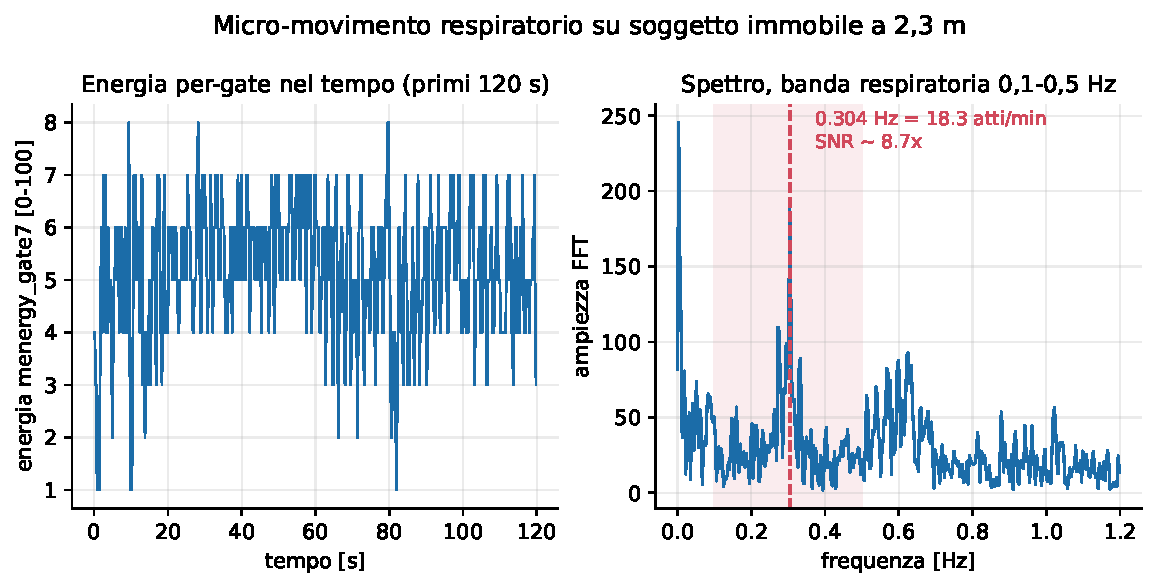
\includegraphics[width=\linewidth]{figures/fig12_respiro}
\caption{Energia per gate di un soggetto immobile a 2,3~m e suo spettro. Il picco
cade in banda respiratoria e canali indipendenti concordano. La verifica contro un
ritmo imposto è nella Tabella~\ref{tab:respiro-metronomo}.}
\label{fig:respiro}
\end{figure}

\subsection{La verifica a ritmo imposto}
\label{sec:respiro-metronomo}

La verifica richiede una ground truth, e il modo più semplice è imporre il ritmo.
Il soggetto è seduto a 2~m rivolto al sensore, perché a 1~m i canali in movimento
saturano, e respira seguendo un metronomo impostato al doppio della frequenza
respiratoria. Sono stati provati tre ritmi, con cinque trial ciascuno da 162~s utili,
più tre trial di stanza vuota come controllo negativo
(Tabella~\ref{tab:respiro-metronomo}).

\begin{table}[htbp]
\centering
\caption{Stima respiratoria contro ritmo imposto, \ldb\ a 2~m. ``Trial concordi''
conta quelli in cui l'analisi ha restituito la fondamentale. }
\label{tab:respiro-metronomo}
\small
\begin{tabular}{@{}lccc@{}}
\toprule
Ritmo imposto & Trial concordi & Stima & Errore \\
\midrule
10 atti/min & 4/5 & $10{,}00 \pm 0{,}00$ & $0{,}00$ \\
15 atti/min & 4/5 & $14{,}95 \pm 0{,}30$ & $-0{,}05$ \\
20 atti/min & 5/5 & $19{,}64 \pm 0{,}09$ & $-0{,}36$ \\
\midrule
Stanza vuota & --- & \multicolumn{2}{c}{\textbf{nessuna stima in 3 trial su 3}} \\
\bottomrule
\end{tabular}
\end{table}

Dove l'analisi identifica la fondamentale la stima è accurata, con errore assoluto
medio di 0,22 atti al minuto sui tredici trial concordi e massimo 0,4. Nei due trial non concordi l'analisi ha restituito
esattamente il doppio del ritmo imposto, mai un valore intermedio, per una ragione
fisica. L'energia per gate risponde all'entità dello spostamento e non al suo verso.
Un ciclo completo (inspirazione ed espirazione) produce quindi due escursioni di
energia e una componente a $2f$ che può superare la fondamentale. La scelta fra $f$ e
$2f$ non è ricavabile dallo spettro di un canale singolo. Il confronto con la ground
truth ha anche corretto due regole di selezione, stabilendo che i gruppi misti di
canali in movimento e stazionari non vanno scartati e che fra due gruppi in rapporto
armonico vince il più basso. Ha inoltre aggiunto una soglia di plausibilità a 8 atti
al minuto, un'assunzione dichiarata che rende il metodo cieco a una respirazione molto
lenta. Le nuove regole non cambiano i risultati precedenti. Restano due limiti. Il
primo è che il metronomo approfondisce il respiro, quindi la validazione riguarda la
frequenza e non l'ampiezza in condizioni realistiche. Il secondo è che sull'esemplare
di \ldc\ lo stesso metodo recupera la frequenza in un trial su tre
(Sezione~\ref{sec:ld2420-risultati}). Il respiro resta quindi una misura dell'\ldb, ed è la
ragione fisica per cui il radar rileva la persona immobile su cui è costruito l'indice
che segue.

\section{Dati di ingresso e algoritmo}
\label{sec:vitalita-ingressi}
\label{sec:vitalita-algoritmo}

L'algoritmo lavora sui campioni a 5~Hz prodotti dal logger e dal firmware della web
UI (Sezione~\ref{sec:c3-4}). Usa l'energia per gate del canale in movimento, la
distanza riportata per scegliere il gate, lo stato di presenza come condizione di
guardia e il rumore di fondo per gate misurato a stanza vuota. Due canali previsti dalla specifica iniziale sono esclusi. Il primo è l'energia stazionaria per gate, nulla sotto 1,5~m (Sezione~\ref{sec:c3-5-2}), e il secondo è l'energia aggregata del bersaglio in movimento. Le ragioni misurate sono ricostruite più avanti, nel paragrafo sulle tre versioni dell'algoritmo.

L'algoritmo ha due componenti, aggiornate a ogni campione $k$, e una fusione. Sia
$e_i[k]$ l'energia in movimento del gate $i$ e $f_i$ il rumore di fondo del gate $i$.

\begin{align}
g^{*} &= \min\!\left(\left\lfloor d_k / 75~\text{cm} \right\rfloor,\; 8\right)
  && \text{gate attivo dalla distanza riportata} \label{eq:gate-attivo}\\
\tilde e_k &= \max\!\left(0,\; \frac{e_{g^{*}}[k] - f_{g^{*}}}{100 - f_{g^{*}}} \cdot 100\right)
  && \text{energia netta, riscalata su 0--100} \label{eq:netta}\\
M_k &= \alpha_m\, \tilde e_k + (1-\alpha_m)\, M_{k-1}
  && \text{livello di movimento, } \alpha_m = 0{,}05 \label{eq:livello}\\
R_k &= \alpha_v\, \left|\tilde e_k - \tilde e_{k-1}\right| + (1-\alpha_v)\, R_{k-1}
  && \text{variabilità del ritorno, } \alpha_v = 0{,}01 \label{eq:variabilita}\\
V_k &= \mathrm{clamp}\!\left(M_k + k\, R_k,\; 0,\; 100\right), \quad k = 0{,}5
  && \text{indice di vitalità} \label{eq:vitalita}
\end{align}

Se il radar non riporta presenza l'indice è 0 e nessuna classe viene assegnata.
Nell'Equazione~\ref{eq:gate-attivo} $d_k$ è la distanza del bersaglio stazionario se
disponibile, altrimenti quella del bersaglio in movimento. In mancanza di entrambe il
gate attivo è quello di massima energia. Le medie esponenziali sono aggiornate su ogni
campione, anche a stanza vuota, così che quando qualcuno entra l'indice non parta da
zero simulando un falso ``nessun segno''.

Ognuna di queste scelte ha una motivazione. Le medie esponenziali costano due variabili
in memoria e girano identiche in Python e in C++, condizione della verifica di
Sezione~\ref{sec:vitalita-bordo}. Le due costanti di tempo sono diverse perché il livello
deve reagire in qualche secondo (a 5~Hz, $\alpha_m = 0{,}05$ vale circa 4~s), mentre
la variabilità è un segnale lento da integrare su circa 20~s. Il fondo va sottratto,
perché senza l'Equazione~\ref{eq:netta} l'indice non distingue una stanza vuota da una persona
immobile. Senza correzione vale infatti 19,1 sulle 6,5~ore di stanza vuota e 17,6 sulla persona immobile a 2,3~m, cioè più a stanza vuota che con la persona, a causa del fondo di 18 e 13 dei gate 0 e 1 di
Tabella~\ref{tab:c3-6}, mentre con la correzione i due casi diventano 2,4 e 15,2. Il gate attivo viene dalla distanza riportata e non
dal massimo di energia, perché sotto il banco i cammini multipli portano energia nei
gate 2--3 mentre la persona è a 60~cm (Sezione~\ref{sec:sotto-banco}). Il peso $k$ fissa il
contributo della variabilità, numericamente piccola, che serve a separare la persona
immobile dal fondo e non a graduare il movimento.

\paragraph{Tre versioni.}
\label{sec:vitalita-evoluzione}
La versione riportata è la terza, e le due precedenti sono state abbandonate per
ragioni misurate. La prima costruiva la componente lenta sulla variazione
dell'energia stazionaria, che nei dati è satura con deviazione standard zero in ogni
scenario occupato, quindi il termine era identicamente nullo. La seconda usava i
canali in movimento, ma definiva il livello come il massimo fra l'energia aggregata
del bersaglio e quella del gate attivo. Tarata a 1~m funzionava, ma sotto il banco
l'energia aggregata satura a 100 e prevale nel massimo qualunque gate si scelga, e con il gate fisso della taratura la persona immobile leggeva 51,1, contro i 28,6 della persona immobile a 1~m. La terza versione usa la sola energia del gate attivo. Gli scenari a 1~m cambiano di pochi punti, mentre quello sotto il banco scende a 25,7 e nei movimenti sotto il banco la saturazione dell'indice si dimezza (Tabella~\ref{tab:vitalita-v2v3}). Con il gate ricavato dalla distanza, adottato dal firmware, la terza versione dà invece 45,4 (la seconda dava 59,2), per la ragione discussa nella Sezione~\ref{sec:vitalita-taratura}.

\begin{table}[htbp]
\centering
\caption{Indice medio per scenario nella seconda e nella terza versione, con la configurazione della taratura (gate fisso~2, fondo della stanza vuota di giorno, parametri tarati). La saturazione è la frazione di campioni con indice a 100.}
\label{tab:vitalita-v2v3}
\small
\begin{tabular}{@{}lrrc@{}}
\toprule
Scenario & v2 & v3 & Saturazione v2 $\to$ v3 \\
\midrule
Immobile, 1~m & 31,1 & 28,6 & 0 $\to$ 0\,\% \\
Micro-movimenti, 1~m & 77,3 & 71,0 & 4 $\to$ 0\,\% \\
Movimento pieno, 1~m & 99,6 & 99,2 & 92 $\to$ 71\,\% \\
\textbf{Immobile sotto il banco} & \textbf{51,1} & \textbf{25,7} & 1 $\to$ 0\,\% \\
\textbf{Movimenti sotto il banco} & 100,0 & \textbf{98,8} & \textbf{100 $\to$ 46\,\%} \\
\bottomrule
\end{tabular}
\end{table}

\section{Classificazione}
\label{sec:vitalita-classi}

Le classi sono tre, non quattro come nella prima specifica, per una ragione
concordata con il relatore. La presenza o assenza non è una classe di vitalità ma la
condizione che sta a monte, perché se il radar non rileva nessuno non c'è nessuno da
classificare. Le classi descrivono quanto si muove chi c'è (Tabella~\ref{tab:vitalita-classi}).

\begin{table}[htbp]
\centering
\caption{Classi dell'indice di vitalità con le soglie tarate
(Sezione~\ref{sec:vitalita-taratura}) e loro significato operativo. }
\label{tab:vitalita-classi}
\small
\begin{tabularx}{\linewidth}{@{}llXl@{}}
\toprule
\textbf{Indice} & \textbf{Classe} & \textbf{Significato operativo} & \textbf{Priorità} \\
\midrule
--- & (nessuna presenza) & il sensore non rileva nessuno & --- \\
0--44 & \texttt{vitalita\_bassa} & presenza confermata, movimento minimo, possibile
  incoscienza & \textbf{la più alta} \\
45--94 & \texttt{vitalita\_moderata} & micro-movimenti, persona che si aggiusta & media \\
95--100 & \texttt{vitalita\_alta} & movimento ampio, persona reattiva & la più bassa \\
\bottomrule
\end{tabularx}
\end{table}

La priorità è il complemento dell'indice, ed è il punto da cui dipende l'interfaccia.
Un segnale debole ma presente significa che c'è qualcuno che non si muove,
possibilmente incosciente, ed è il caso da raggiungere per primo. Un segnale forte
significa che c'è qualcuno che si muove, probabilmente cosciente e in grado di
aspettare. Per questo nella dashboard (Sezione~\ref{sec:webui-progetto}) la classe bassa è
rossa e la classe alta verde. Le classi sono un supporto informativo al triage e non
una diagnosi medica. Vitalità bassa significa che il sensore rileva una presenza con
variazioni minime, non che la persona è in pericolo di vita. L'assenza di presenza
significa che il sensore non rileva nessuno, non che nessuno è vivo, perché la persona
può essere fuori portata, schermata da metallo o priva di sensi ma viva.

\section{Taratura e validazione}
\label{sec:vitalita-taratura}

L'algoritmo si sviluppa su PC, sui file CSV, e il porting su ESP32 avviene solo a
parametri validati. I dati esistono già dalla campagna del Capitolo~\ref{chap:confronto}. La
dose-risposta di Sezione~\ref{sec:dose-risposta} copre i tre scenari a geometria costante
(1~m in piedi, cinque trial ciascuno, immobile, micro-movimenti, cammino sul posto).
Le due serie sotto il banco (Sezione~\ref{sec:sotto-banco}) sono l'insieme di validazione su
geometria diversa. Il fondo per gate della taratura viene dalla stanza vuota di giorno, quello del firmware dalla notte (Sezione~\ref{sec:vitalita-bordo}). I parametri
($\alpha_m$, $\alpha_v$, $k$ e le due soglie) sono stati scelti sui trial T01--T03
dei tre scenari a 1~m, collocando le soglie negli intervalli fra le distribuzioni
dell'indice per scenario. La prestazione è misurata sui trial T04--T05, mai usati per
la scelta. La metrica è la recall per classe, cioè la percentuale di campioni di ogni
scenario che cadono nella classe attesa, mediata sulle classi, e il transitorio è
scartato come nel Capitolo~\ref{chap:confronto}. Nella taratura il gate attivo era fissato al
gate~2 anziché ricavato dalla distanza, perché a 1~m la persona sta a cavallo dei
gate 1 e 2 e il gate~2 ha il fondo più pulito. La conseguenza di questa scelta è
discussa sotto.

\begin{table}[htbp]
\centering
\caption{Prestazione dell'indice a tre classi con i parametri tarati e gate fisso 2. La recall è media per classe e per campione.}
\label{tab:vitalita-validazione}
\small
\begin{tabular}{@{}lc@{}}
\toprule
Insieme & Recall media \\
\midrule
Taratura (T01--T03, 1~m) & $95{,}1\,\%$ \\
Validazione (T04--T05, 1~m) & $\mathbf{88{,}0\,\%}$ \\
Validazione su geometria diversa (sotto il banco) & $51{,}2\,\%$ \\
\midrule
Discriminazione immobile / in movimento, entrambe le geometrie & $\mathbf{96{,}1\,\%}$ \\
\bottomrule
\end{tabular}
\end{table}

\begin{table}[htbp]
\centering
\caption{Dettaglio per scenario con i parametri tarati, tutti i trial, gate fisso 2 e fondo della stanza vuota di giorno.
L'indice è la media dell'indice medio per trial. }
\label{tab:vitalita-scenari}
\small
\begin{tabular}{@{}lrlr@{}}
\toprule
Scenario & Indice & Classe attesa & Corretti \\
\midrule
Immobile a 1~m & 28,6 & bassa & $89{,}9\,\%$ \\
Micro-movimenti a 1~m & 71,0 & moderata & $90{,}5\,\%$ \\
Movimento pieno a 1~m & 99,2 & alta & $96{,}3\,\%$ \\
Immobile sotto il banco & 25,7 & bassa & $97{,}5\,\%$ \\
Movimenti sotto il banco & 98,8 & moderata & $4{,}8\,\%$ \\
\bottomrule
\end{tabular}
\end{table}

\begin{figure}[htbp]
\centering
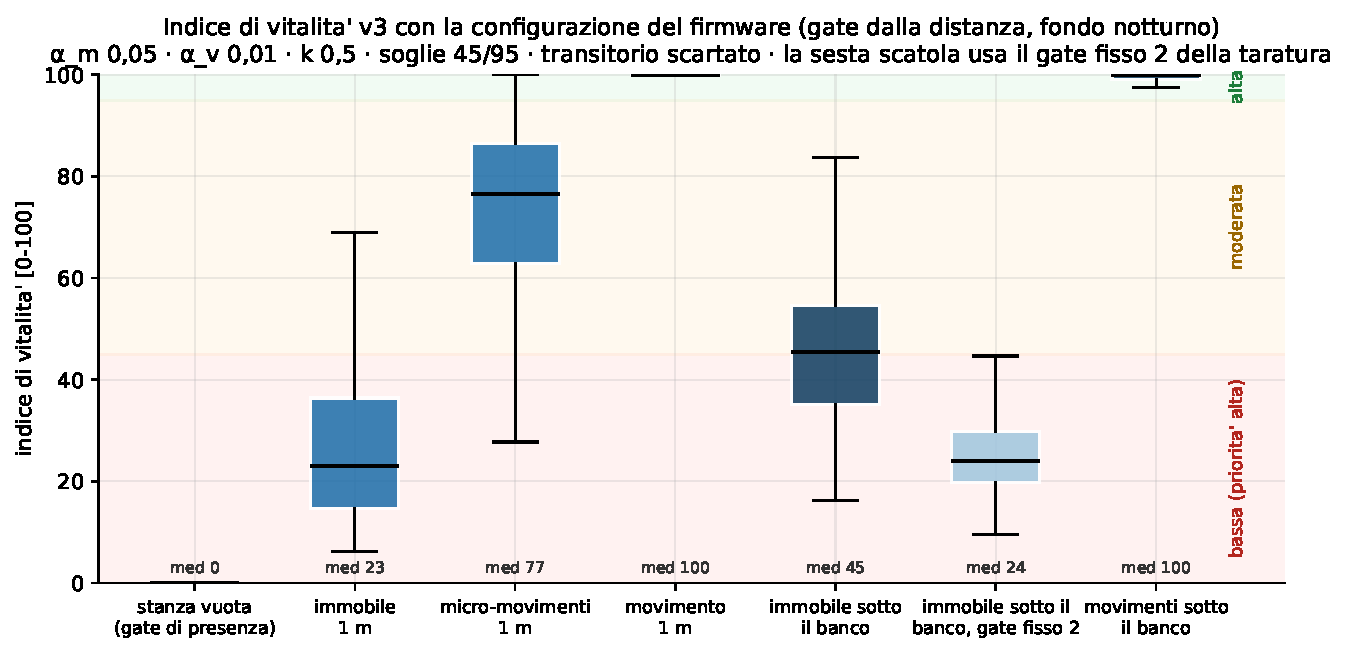
\includegraphics[width=\linewidth]{figures/fig21_vitalita_scenari}
\vspace{2.6cm}% spazio per la didascalia nel margine
\caption{Distribuzione dell'indice di vitalità v3 per scenario, con la configurazione
del firmware (gate dalla distanza riportata, fondo notturno), transitorio scartato.
Le fasce colorate sono le tre classi. Le tre scatole a 1~m si separano. Sotto il banco
la persona immobile dà mediana 45, a cavallo della soglia bassa/moderata. La sesta
scatola ripete lo scenario con il gate fissato a 2, come nella taratura. La mediana
scende a 24, per la ragione discussa nel testo.}
\label{fig:vitalita-scenari}
\end{figure}

\paragraph{Sulla geometria di taratura.} Sui trial di validazione a 1~m l'indice
classifica correttamente l'88\,\% dei campioni su scenari mai visti in fase di
taratura (Tabelle~\ref{tab:vitalita-validazione} e~\ref{tab:vitalita-scenari}). Le tre distribuzioni
si separano (Figura~\ref{fig:vitalita-scenari}), con mediane 23, 77 e 100. La
sovrapposizione è concentrata fra la persona immobile e quella che compie piccoli
movimenti, la stessa zona in cui il PIR era imprevedibile (Sezione~\ref{sec:dose-risposta}).

\paragraph{Sulla geometria diversa.} Il 51,2\,\% sotto il banco è dominato da un
solo scenario. Fra i quattro corretti c'è la persona immobile, riconosciuta nel
97,5\,\% dei campioni. Sarebbe tentante presentarlo come prova che le soglie si
trasferiscono alla geometria del progetto, ma non lo è. La ragione sta nel gate
fissato a~2. Sotto il banco la persona è a 60~cm, cioè nel gate~1, e il gate~2
raccoglie soltanto un'eco indiretta (Tabella~\ref{tab:vitalita-gate}). Il 25,7 nasce da un
gate in cui la persona non è, e vale quanto l'immobile a 1~m per coincidenza. Letta
nel suo gate, la stessa persona immobile ha energia 54, quanto i micro-movimenti a
1~m. Con il criterio a distanza l'indice vale 45,4 ed è in classe bassa nel 49\,\% dei
campioni. Il dato che si trasferisce davvero è la discriminazione fra immobile e in
movimento, con il 96,1\,\% di recall su tutti e cinque gli scenari e su entrambe le
geometrie, netta con qualunque criterio di gate. Ed è la distinzione che conta per il
triage, perché separa chi è presente e immobile, con la massima priorità, da chi è
presente e in movimento. Il caso che fallisce sono i movimenti sotto il banco,
classificati alta anziché moderata, ma l'etichetta attesa era stata assegnata per
analogia con il caso a 1~m, senza ground truth indipendente. Poiché a 60~cm una
persona che si aggiusta produce un ritorno molto forte, il dato onesto è che l'indice
colloca quello scenario in alto, non che sbagli.

\begin{table}[htbp]
\centering
\caption{Energia in movimento media grezza per gate nei cinque scenari. A 60~cm la
persona sta nel gate~1. Il gate~2 usato dalla taratura ne vede solo l'eco indiretta.}
\label{tab:vitalita-gate}
\small
\begin{tabular}{@{}lrrrr@{}}
\toprule
Scenario & Gate 0 & Gate 1 & Gate 2 & Gate 3 \\
\midrule
Stanza vuota (fondo) & 17,6 & 13,2 & 4,4 & 2,9 \\
Immobile a 1~m & 18,6 & 30,9 & 25,3 & 7,4 \\
Micro-movimenti a 1~m & 23,6 & 66,5 & 60,5 & 14,3 \\
\textbf{Immobile sotto il banco (60~cm)} & 33,1 & \textbf{54,0} & 21,7 & 9,5 \\
Movimenti sotto il banco & 96,5 & 99,8 & 95,1 & 43,9 \\
\bottomrule
\end{tabular}
\end{table}

Le soglie restano quindi specifiche della geometria in cui sono state tarate. Il gate
fisso non è una soluzione, ma un modo di nascondere il problema. Per il progetto è
gestibile, perché ogni sensore è montato in posizione fissa sotto il proprio arredo e
può essere tarato una volta in quella posizione, mentre sarebbe un problema per un
dispositivo portatile.

\section{Porting a bordo e verifica}
\label{sec:vitalita-bordo}

Su richiesta del relatore l'indice è calcolato a bordo del nodo e mostrato nella
dashboard (Sezione~\ref{sec:webui}). Le
Equazioni~\ref{eq:gate-attivo}, \ref{eq:netta}, \ref{eq:livello}, \ref{eq:variabilita} e~\ref{eq:vitalita} sono
implementate in 74 righe di C++ senza dipendenze, con le stesse costanti del prototipo
in un unico file di configurazione. Il costo è di poche operazioni in virgola mobile
per campione. Il firmware usa il gate dalla distanza riportata. A 1~m riproduce la taratura (28,4, 73,9 e 99,4 contro 28,6, 71,0 e 99,2 con il gate fisso), e sotto il banco legge il gate in cui il radar colloca davvero la persona (Sezione~\ref{sec:vitalita-taratura}), così che la dipendenza dalla geometria è dichiarata anziché nascosta. Il fondo per gate è quello della stanza vuota notturna di
6,5~ore, e la scelta del file di fondo sposta l'indice di meno di un punto.

Il criterio di accettazione era che l'indice calcolato sull'ESP32 e quello calcolato
in Python sullo stesso CSV coincidessero entro l'arrotondamento. Il firmware scrive
indice e classe in due colonne supplementari del CSV esportato dal browser
(Sezione~\ref{sec:webui-progetto}), e uno script di confronto rilegge il file con il
prototipo campione per campione. Le sessioni sono sei, da 90~s, con soggetto immobile, con
micro-movimenti e in movimento, a circa 1,9~m e a 1~m. A regime i due indici
coincidono entro $\pm 1$ nel 98,7--100\,\% dei campioni (Figura~\ref{fig:vitalita-bordo}).
Nei primi 60~s circa divergono per una ragione strutturale. Le medie esponenziali del
firmware partono dall'accensione del nodo e sono già a regime quando la sessione
inizia, mentre quelle del prototipo partono dal primo campione del file. La divergenza
iniziale conferma che le due implementazioni sono la stessa funzione applicata a stati
iniziali diversi.

\begin{figure}[htbp]
\centering
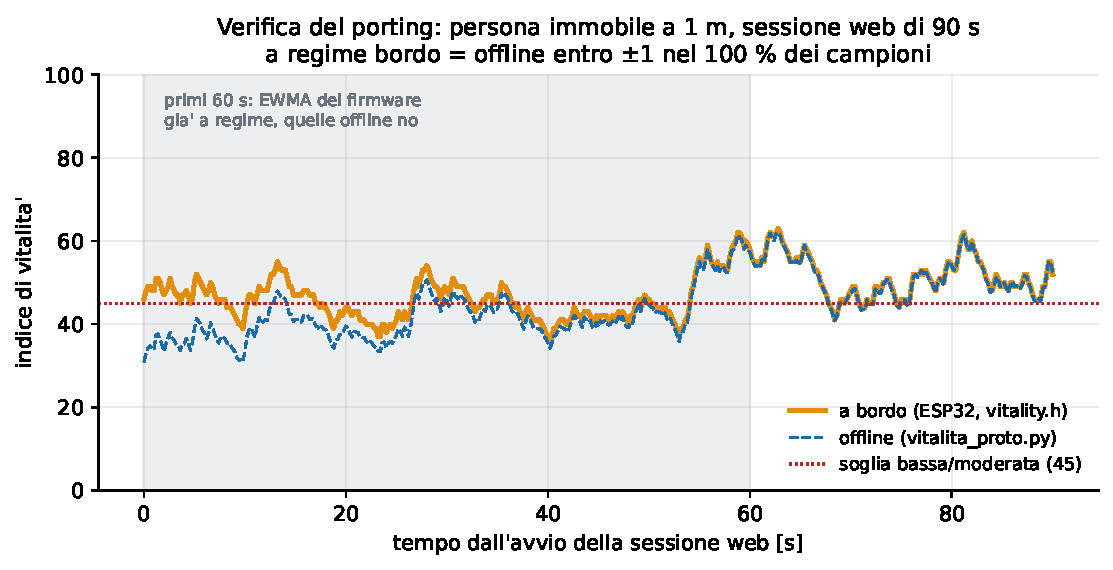
\includegraphics[width=\linewidth]{figures/fig22_vitalita_bordo}
\caption{Verifica del porting, con l'indice calcolato a bordo dell'ESP32 e il
ricalcolo offline sullo stesso CSV esportato dalla web UI per una persona immobile a
1~m. Nei primi
60~s le medie esponenziali offline devono ancora convergere. Dopo, le due curve
coincidono entro $\pm 1$ nel 100\,\% dei campioni.}
\label{fig:vitalita-bordo}
\end{figure}

Le sessioni dal vivo sono una dimostrazione del funzionamento a bordo, non una
seconda validazione delle soglie. A 1,9~m le tre condizioni hanno dato 19,9 (bassa),
68,7 (moderata) e 94,0, e l'ultimo valore sta a cavallo della soglia 95 tarata a 1~m,
un'altra manifestazione della dipendenza dalla geometria. A 1~m gli indici sono stati
47,7, 99,4 e 99,1, con i micro-movimenti classificati alta. Il gate~1 grezzo (97,9,
canale in movimento attivo nel 99\,\% dei campioni) mostra però che lo stimolo di
quella sessione era un movimento pieno, non i micro-movimenti della serie di taratura
(66--68, canale attivo nel 72\,\%). L'indice ha quindi letto correttamente lo stimolo
che ha ricevuto, ed è la condizione ``micro-movimenti'' a dipendere dall'operatore e a
non riprodursi fra sessioni.

\section{Limiti, casi limite ed estensioni}
\label{sec:vitalita-limiti}

La stessa costruzione non è applicabile all'\ldc. Sull'esemplare in dotazione la
dose-risposta è piatta e rovesciata (Sezione~\ref{sec:ld2420-risultati}), e non esiste la
grandezza continua da cui l'indice si calcola. L'obbiettivo O6 resta sull'\ldb, come
limite dell'esemplare e non del modello. I comportamenti dell'indice nei casi limite
sono raccolti in Tabella~\ref{tab:vitalita-casilimite}.

\begin{table}[htbp]
\centering
\caption{Casi limite dell'indice di vitalità e comportamento previsto o osservato.}
\label{tab:vitalita-casilimite}
\small
\begin{tabularx}{\linewidth}{@{}XXX@{}}
\toprule
\textbf{Situazione} & \textbf{Comportamento} & \textbf{Note} \\
\midrule
La persona esce dal campo & indice a 0 e nessuna classe entro la coda di presenza
  del radar (circa 9--12~s stimati, Sezione~\ref{sec:latenza}) & forzatura sulla condizione di
  presenza. Le medie continuano ad aggiornarsi \\
La persona si addormenta & da alta a bassa in qualche decina di secondi & le medie
  esponenziali decadono con le loro costanti (4 e 20~s) \\
Ventilatore o tenda in movimento & possibile falsa classe moderata & limite da
  dichiarare. Mitigazione tramite le soglie per gate del radar \\
Due persone & indice riferito al gate della distanza riportata & coerente con il
  limite di un bersaglio per canale (Sezione~\ref{sec:due-persone}) \\
Persona oltre 4--5~m & energia debole, indice sottostimato & la portata utile
  dell'indice non è stata caratterizzata \\
Persona a meno di 1,5~m & nessun effetto, l'indice usa i soli canali in movimento &
  scelta imposta da Sezione~\ref{sec:c3-5-2} \\
\bottomrule
\end{tabularx}
\end{table}

I limiti dell'indice, nell'ordine in cui pesano, sono quattro. Il primo è che le
soglie sono specifiche dell'installazione. Il secondo è che la validazione poggia su
un solo soggetto e due trial per scenario. Il terzo è la mancanza di una ground truth
indipendente per la classe intermedia, e il quarto è che la portata utile non è
caratterizzata. Sono state inoltre individuate tre estensioni, non necessarie
all'obbiettivo. L'auto-taratura all'installazione, che registri il fondo a stanza vuota e un riferimento di movimento sotto l'arredo, è la prima da fare, perché risolve il limite principale. La seconda è un'isteresi sulle classi, che farebbe cambiare
un'etichetta solo dopo qualche secondo di stabilità, così che non sfarfalli quando
l'indice oscilla intorno a una soglia, come nella sessione a 1,9~m. La terza è un
indicatore di confidenza affiancato all'indice, funzione della stabilità del gate
attivo, che direbbe quanto fidarsi del valore. La sostituzione della componente lenta
con una potenza in banda respiratoria, ipotizzata nella prima specifica, non è invece
più fra le priorità, per la scelta di formulazione della Sezione~\ref{sec:vitalita-motivazione}.

Resta infine un aspetto di trattamento dei dati. Per il monitoraggio in ambienti scolastici il progetto indica le cautele del GDPR, fino a una valutazione d'impatto quando sono coinvolti minori~\cite{callisto2026dipme}. L'indice di vitalità non aggiunge un problema nuovo, perché è una misura generica di quanto si muove chi è presente e non una misura fisiologica (Sezione~\ref{sec:vitalita-motivazione}). Rientra quindi nella stessa valutazione che riguarda già il dato di presenza.
